\documentclass{VUMIFPSkursinis}
\usepackage{algorithmicx}
\usepackage{algorithm}
\usepackage{algpseudocode}
\usepackage{amsfonts}
\usepackage{amsmath}
\usepackage{bm}
\usepackage{caption}
\usepackage{color}
\usepackage{float}
\usepackage{graphicx}
\usepackage{listings}
\usepackage{subfig}
\usepackage{wrapfig}
\usepackage{sectsty}

\usepackage{enumitem}
%PAKEISTA, tarpai tarp sąrašo elementų
\setitemize{noitemsep,topsep=0pt,parsep=0pt,partopsep=0pt}
\setenumerate{noitemsep,topsep=0pt,parsep=0pt,partopsep=0pt}
\allsectionsfont{\centering}
% Titulinio aprašas
\university{Vilniaus universitetas}
\faculty{Matematikos ir informatikos fakultetas}
\department{Programų sistemų katedra}
\papertype{Programų sistemų inžinerijos I laboratorinis darbas}
\title{Socialinis Vilniaus universiteto tinklalapis}
\titleineng{SocialVU}
\status{2 kurso 4 grupės studentai}
\author{Andrejus Voitovas}
\secondauthor{Eglė Puodžiūnaitė}
\thirdauthor{Kasparas Kralikas}
\fourthauthor{Ieva Vizgirdaitė} % Pridėti antrą autorių
\supervisor{asist. dr. Vytautas Valaitis}
\date{Vilnius – \the\year}

% Nustatymai
% \setmainfont{Palemonas}   % Pakeisti teksto šriftą į Palemonas (turi būti įdiegtas sistemoje)
\bibliography{bibliografija}

\begin{document}
% PAKEISTA
\maketitle
\cleardoublepage\pagenumbering{arabic}
\setcounter{page}{2}
\sectionnonum{ANOTACIJA}
Šiame dokumente pateikiami funkciniai ir nefunkciniai reikalavimai sistemai. Sistema ana-
lizuojama taikant ICONIX metodą. Apibrėžiamas struktūrinis dalykinės srities modelis, paaiški-
namos sistemoje naudojamos sąvokos. Taip pat aprašomos sistemoje atliekamos užduotys, anali-
zuojami pagrindiniai ir alternatyvūs užduoties scenarijai, naudojant sekų diagramas. Apibrėžiama
techninė kuriamos sistemos architektūra bei testavimo planas ir scenarijai. Kuriamos sistemos architektūra aprašoma naudojant UML 4+1 požiūrių
rinkinį. Žvelgiama į sistemą 5 skirtingais požiūriais. Loginis pjūvis skirtas parodyti sistemos
funkcionalumą, aprašyti santykius tarp esybių. Užduočių pjūvyje pateiksime, kokias užduotis gali
įgyvendinti naudotojas, kokie jų įgyvendimo scenarijai. Kūrimo pjūvyje pateikiama, kaip susiję atskiri
komponentai. Fiziniame pjūvyje parodoma, kaip sistema išdėstoma tinkle, kaip ji diegiama,
kokia įranga naudojama. Procesų pjūvis pateikia dinaminį sistemos modelį: paaiškina sistemoje
vykstančius procesus, parodo, kaip procesai komunikuoja, galimus sistemos darbo atvejus.
\newpage
%TURINYS
\tableofcontents
\begin{center}
\sectionnonum{ĮVADAS}
\end{center}
\textbf{Tikslas}  - sukurti socialinio tinklalalapio prototipą, kurį įgyvendinus būtų palengvinta universiteto bendruomenės komunikaciją.\\
\textbf{Temos aktualumas} \\
Šiuo metu studentams dėstytojų skelbiama informacija yra išbarstyta internete, kurią surasti užima galybes laiko. Yra atskiras universiteto naujienų puslapis, kiekvienas dėstytojas turi savo asmeninį tinklalapį, atskiras elektroninis paštas. Tiek dėstytojui pasiekti studentus, tiek studentui dėstytoją yra komplikuota ir nepatogu.\\
\textbf{Dalykinė sritis}\\
Socialinis Vilniaus Universiteto tinklapis.\\
\textbf{Probleminė sritis}\\
Socialinis Vilniaus Universiteto tinklapis suteiktų galimybę greitai ir paprastai pasiekti šio universiteto dėstytojų puslapius, informaciją juose, susisiekti sus pačiais dėstytojais. Pagrindinis tinklalapio išskirtinumas - greitai ir patogiai pasiekiama informacija, viskas vienoje vietoje. Itin patogus valdymas dėstytojams.\\
 \textbf{Naudoti dokumentai}\\
 Dokumentas parengtas pagal kursinio darbo reikalavimus naudojant Latex programą ir jau sukurtus šablonus.\\
 \textbf{Darbo pagrindas} \\ 
Dokumentas parengtas kaip Programų sistemų inžinerijos I laboratorinis darbas.
\newpage
\section{LOGINIS PJŪVIS}
Loginį pjūvį sudaro klasių diagramos, kurios naudojamos pavaizduoti sistemos architektūros projektavimo etapus.
\subsection{Esybių klasių diagrama (nulinis lygis)}
\begin{figure}[H]
\centering
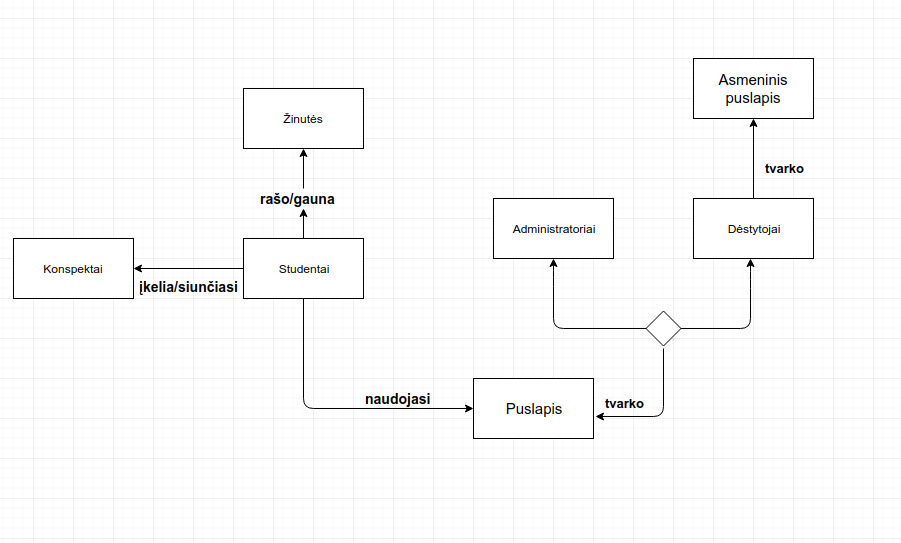
\includegraphics[width=\linewidth]{img/dalykine.png}
\caption{Dalykinė srities UML diagrama}
\label{fig:dalykine}
\end{figure}
\ref{fig:dalykine} pav. esybių diagramoje vaizduojamos esybių sąsajos. Pagrindinė esybė Naudotojas,
kuris gali būti Studentas, Dėstytojas arba Administratorius. Studentas turi galimybę naudotis pagrindinėmis puslapio funkcijos, o dėstytojai ir administratoriai pateikti naudingą studentams meždiagą. Taip pat studentai bei dėstytojai gali komunikuoti tarpusavyje nesinaudojant trečiųjų šalių komunikacinėmis priemonėmis. Administratoriai, savo ruožtu, pateikia informaciją apie renginius, naujienas ir D.U.K.
\subsection{Klasių diagrama (pirmas lygis)}
\begin{figure}[H]
\centering
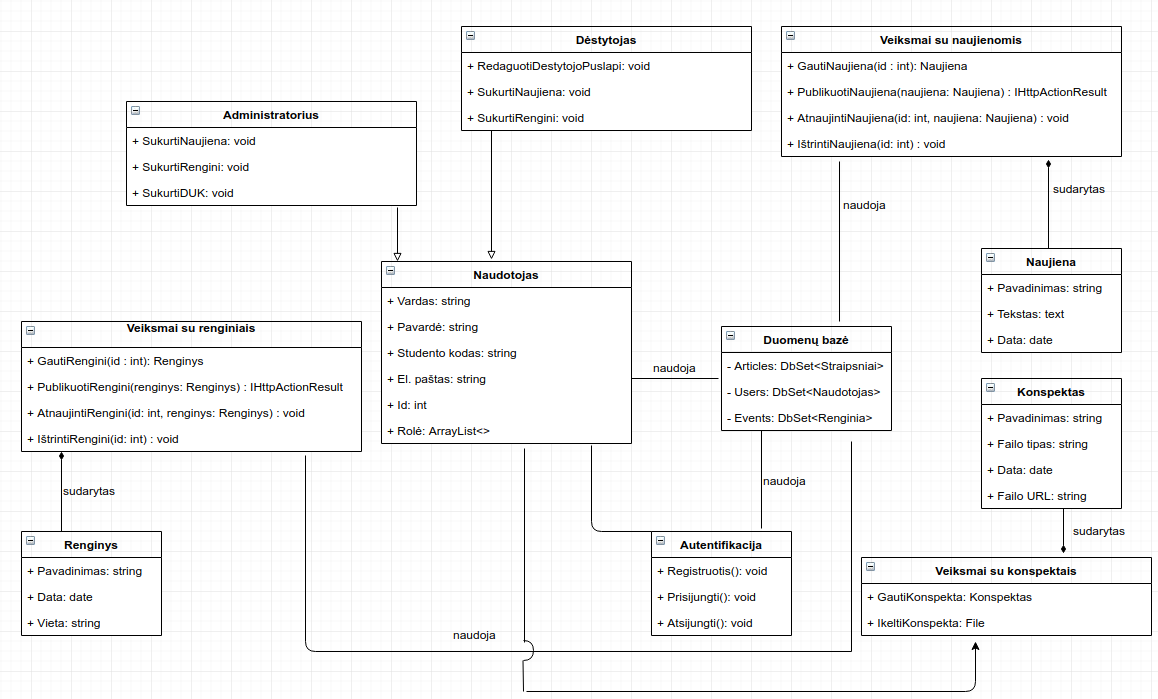
\includegraphics[width=\linewidth]{img/pagrindine.png}
\caption{Dalykinė srities UML diagrama}
\label{fig:pagrindine}
\end{figure}
Pagrindinį programos funkcionalumą užtikrina šios klasės: Studentas, Dėstytojas, Administratorius, Reitingas, Dėsytotojo puslapis, Naujienos, Autentifikacija, Duomenų bazė,
D.U.K., Renginiai. Veikimą įgyvendinačių klasių tarpusavio bendradarbiavimas vaizduojamas asociacija, ge-
neralizacija, kompozicija bei kardinalumus (\ref{fig:pagrindine}  pav.).
\newpage
\section{UŽDUOČIŲ PJŪVIS}
Šiame skyriuje aprašomas kuriamo socialinio tinklalapio galimi panaudojimo atvejai. Pasinaudojant užduočių diagrama pateikiami studento ir dėstytojo (SocialVU naudotojų) tikslai socialiniam tinklalapiui. Kiekvienai užduočiai pateikiamas scenarijus, kuris parodo, kaip užduotis įgyvendinama.
\subsection{Sistemoje vykdomos užduotys}
\begin{figure}[H]
\centering
\includegraphics[width=\linewidth]{img/socpslSistema.png}
\caption{Socialiniame tinklalapyje vykdomos užduotys}
\label{fig:socpslsist}
\end{figure}
Sistemoje vykdomos pagrindinės užduotys: studentas gali peržiūrėti pasirinkto dėstytojo puslapius. Dėstytojams sudaroma galimybė pateikti aktualias naujienas, informaciją apie renginius, redaguoti savo asmeninius tinklalapius, kuriuose gali talpinti informaciją apie savo dėstomus dalykus bei kitą naudingą informaciją, kurią matys jų studentai. Tiek dėstytojai, tiek studentai gali gauti informaciją apie juos dominančius renginius, matyti aktualias naujienas, gauti bei siųsti žinutes.(\ref{fig:socpslsist} pav.).
\subsection{Užduočių vykdymo scenarijai}
Užduočių vykdymo scenarijai, atvaizduoja agentų, šiuo atveju studento ir dėstytojo, įmanomų įvykdyti užduočių veiksmus paeiliui , nuo pradžios iki užduoties vykdymo pabaigos.
\subsection{Užduoties "Pridėti naujieną" scenarijus}
\begin{figure}[H]
	\centering
	\includegraphics[scale=0.65]{img/addNew.png}
	\caption{Užduoties "Pridėti naujieną" scenarijus}
	\label{fig:addNew}
\end{figure}
\textbf{Žingsnių seka (\ref{fig:addNew}pav.)}\\
\begin{enumerate}
	\item Sukurti naujieną - dėstytojas paspaudžia ant nuorodos leidžiančios sukurti naujieną.
	\item Informacija apie naujieną? - naujienų UI išmeta dėstytojui naujienos formą užpildymui.
	\item Naujienos informacija - naudotojas išsiunčia užpildytą formą naujienų UI.
	\item Sukurti naujieną - įvesta naujienos informacija yra siunčiama kontroleriui.
	\item Pridėti naujieną - darbų UI įdeda naujieną į duomenų bazę.
	\item Naujiena pridėta - duomenų bazė parsiunčia naujienos patalpinimo patvirtinimą.
	\item Gauti naujienų sąrašą - naujienų kontroleris prašo duomenų bazės pateikti naują naujienų sąrašą.
	\item Naujienų sąrašas - naujienų sąrašas keliauja iš duomenų bazės iki dėstytojo.
\end{enumerate}
\subsection{Užduoties "Ištrinti naujieną" scenarijus}
\begin{figure}[H]
	\centering
	\includegraphics[scale=0.65]{img/deleteNew.png}
	\caption{Užduoties "Ištrinti naujieną" scenarijus}
	\label{fig:delNew}
\end{figure}
\textbf{Žingsnių seka (\ref{fig:delNew}pav.)}\\
\begin{enumerate}
	\item Ištrinti naujieną - dėstytojas paspaudžia nuorodą ištrinančią naujieną.
	\item Patvirtinti ištrynimą? - naudotojas prašomas patvirtinti ištrynimą.
	\item Patvirtinti ištrynimą - dėstytojas patvirtina ištrynimą.
	\item Ištrinti naujieną - pateikiama naujiena ištrynimui įvykdyti.
	\item Ištrinti naujieną - prašoma duomenų bazės surasti ir ištrinti naujieną.
	\item Gauti naujienų sąrašą - siunčiamas prašymas naujienų sąrašui gauti iš duomenų bazės.
	\item Naujienų sąrašas - atnaujintas sąrašas keliauja iki dėstytojo.
\end{enumerate}
\subsection{Užduoties "Redaguoti naujieną" scenarijus}
\begin{figure}[H]
	\centering
	\includegraphics[scale=0.65]{img/editNew.png}
	\caption{Užduoties "Redaguoti naujieną" scenarijus}
	\label{fig:edNew}
\end{figure}
\textbf{Žingsnių seka (\ref{fig:edNew}pav.)}\\
\begin{enumerate}
	\item Redaguoti naujieną - dėstytojas paspaudžia nuorodą leidžiančią redaguoti naujieną.
	\item Redaguoti naujieną - pateikiama naujiena naujienų kontroleriui.
	\item Surasti naujieną - naujiena ieškoma duomenų bazėje.
	\item Naujiena - duomenų bazė pateikia naujieną kontroleriui.
	\item Naujienos informacija -  informacija apie naujieną keliauja iki naudotojo.
	\item Naujienos informacija - informacija apie naujieną keliauja iki naudotojo.
	\item Išsaugoti pakeitimus - naudotojas prašo išsaugoti įvykdytus pakeitimus.
	\item Redaguoti naujieną - naujiena siunčiama redagavimui.
	\item Išsaugoti pakeitimus - pakeitimai išsaugomi duomenų bazėje.
	\item Gauti naujienų sąrašą - kontroleris prašo duomenų bazės gauti atnaujintą naujienų sąrašą.
	\item Naujienų sąrašas - naujienų sąrašas keliauja iš duomenų bazės iki dėstytojo.
\end{enumerate}
\subsection{Užduoties "Peržiūrėti naujienas" scenarijus}
\begin{figure}[H]
	\centering
	\includegraphics[scale=0.65]{img/viewNew.png}
	\caption{Užduoties "Peržiūrėti naujienas" scenarijus}
	\label{fig:viewNew}
\end{figure}
\textbf{Žingsnių seka (\ref{fig:viewNew}pav.)}\\
\begin{enumerate}
	\item Gauti naujienų sąrašą - dėstytojas paspaudžia nuorodą į naujienų sąrašą.
	\item Gauti naujienų sąrašą - prašymas gauti naujienų sąrašą keliauja iki duomenų bazės.
	\item Naujienų sąrašas - naujienų sąrašas iš duomenų bazės keliauja iki naudotojo.
\end{enumerate}
\subsection{Užduoties "Pridėti renginį" scenarijus}
\begin{figure}[H]
	\centering
	\includegraphics[scale=0.65]{img/addNewEvent.png}
	\caption{Užduoties "Pridėti renginį" scenarijus}
	\label{fig:addNewEvent}
\end{figure}
\textbf{Žingsnių seka (\ref{fig:addNewEvent}pav.)}\\
\begin{enumerate}
	\item Sukurti renginį - dėstytojas paspaudžia ant nuorodos leidžiančios sukurti renginį.
	\item Informacija apie renginį? - renginių UI išmeta dėstytojui renginio formą užpildymui.
	\item Renginio informacija - naudotojas išsiunčia užpildytą formą renginių UI.
	\item Sukurti renginį - įvesta renginio informacija yra siunčiama kontroleriui.
	\item Pridėti renginį - renginių UI įdeda renginį į duomenų bazę.
	\item Renginys pridėtas - duomenų bazė parsiunčia renginio patalpinimo patvirtinimą.
	\item Gauti renginių sąrašą - renginių kontroleris prašo duomenų bazės pateikti naują renginių sąrašą.
	\item Renginių sąrašas - renginių sąrašas keliauja iš duomenų bazės iki dėstytojo.
\end{enumerate}
\subsection{Užduoties "Ištrinti renginį" scenarijus}
\begin{figure}[H]
	\centering
	\includegraphics[scale=0.65]{img/deleteEvent.png}
	\caption{Užduoties "Ištrinti renginį" scenarijus}
	\label{fig:delEvent}
\end{figure}
\textbf{Žingsnių seka (\ref{fig:delEvent}pav.)}\\
\begin{enumerate}
	\item Ištrinti renginį - dėstytojas paspaudžia nuorodą ištrinančią renginį.
	\item Patvirtinti ištrynimą? - naudotojas prašomas patvirtinti ištrynimą.
	\item Patvirtinti ištrynimą - dėstytojas patvirtina ištrynimą.
	\item Ištrinti renginį - pateikiamas renginys ištrynimui įvykdyti.
	\item Ištrinti renginį - prašoma duomenų bazės surasti ir ištrinti renginį.
	\item Gauti renginių sąrašą - siunčiamas prašymas renginių sąrašui gauti iš duomenų bazės.
	\item Renginių sąrašas - atnaujintas sąrašas keliauja iki dėstytojo.
\end{enumerate}
\subsection{Užduoties "Redaguoti renginį" scenarijus}
\begin{figure}[H]
	\centering
	\includegraphics[scale=0.65]{img/editEvent.png}
	\caption{Užduoties "Redaguoti renginį" scenarijus}
	\label{fig:editEvent}
\end{figure}
\textbf{Žingsnių seka (\ref{fig:editEvent}pav.)}\\
\begin{enumerate}
	\item Redaguoti renginį - dėstytojas paspaudžia nuorodą leidžiančią redaguoti renginį.
	\item Redaguoti renginį - pateikiamas renginys renginių kontroleriui.
	\item Surasti renginį - renginys ieškomas duomenų bazėje.
	\item Renginys - duomenų bazė pateikia renginį kontroleriui.
	\item Renginio informacija -  informacija apie renginį keliauja iki naudotojo.
	\item Renginio informacija - informacija apie renginį keliauja iki naudotojo.
	\item Išsaugoti pakeitimus - naudotojas prašo išsaugoti įvykdytus pakeitimus.
	\item Redaguoti renginį - renginys siunčiamas redagavimui.
	\item Išsaugoti pakeitimus - pakeitimai išsaugomi duomenų bazėje.
	\item Gauti renginių sąrašą - kontroleris prašo duomenų bazės gauti atnaujintą renginių sąrašą.
	\item Renginių sąrašas - renginių sąrašas keliauja iš duomenų bazės iki dėstytojo.
\end{enumerate}
\subsection{Užduoties "Peržiūrėti renginius" scenarijus}
\begin{figure}[H]
	\centering
	\includegraphics[scale=0.65]{img/viewEvent.png}
	\caption{Užduoties "Peržiūrėti renginius" scenarijus}
	\label{fig:viewEvent}
\end{figure}
\textbf{Žingsnių seka (\ref{fig:viewEvent}pav.)}\\
\begin{enumerate}
	\item Gauti renginių sąrašą - dėstytojas paspaudžia nuorodą į renginių sąrašą.
	\item Gauti renginių sąrašą - prašymas gauti renginių sąrašą keliauja iki duomenų bazės.
	\item Renginių sąrašas - renginių sąrašas iš duomenų bazės keliauja iki naudotojo.
\end{enumerate}
\subsection{Užduoties "Pridėti D.U.K." scenarijus}
\begin{figure}[H]
	\centering
	\includegraphics[scale=0.65]{img/addDUK.png}
	\caption{Užduoties "Pridėti D.U.K." scenarijus}
	\label{fig:addDuk}
\end{figure}
\textbf{Žingsnių seka (\ref{fig:addDuk}pav.)}\\
\begin{enumerate}
	\item Pridėti D.U.K. - dėstytojas paspaudžia ant nuorodos leidžiančios sukurti D.U.K.
	\item Informacija apie klausimą? - D.U.K. UI išmeta dėstytojui D.U.K. formą užpildymui.
	\item Klausimo informacija - naudotojas išsiunčia užpildytą formą D.U.K. UI.
	\item Sukurti  klausimą - įvesta klausimo informacija yra siunčiama kontroleriui.
	\item Pridėti klausimą - D.U.K. UI įdeda klausimą į duomenų bazę.
	\item Klausimas pridėtas - duomenų bazė parsiunčia klausimo patalpinimo patvirtinimą.
	\item Gauti D.U.K. sąrašą - D.U.K. kontroleris prašo duomenų bazės pateikti naują D.U.K. sąrašą.
	\item D.U.K. sąrašas - D.U.K. sąrašas keliauja iš duomenų bazės iki dėstytojo.
\end{enumerate}
\subsection{Užduoties "Peržiūrėti D.U.K." scenarijus}
\begin{figure}[H]
	\centering
	\includegraphics[scale=0.65]{img/viewDUK.png}
	\caption{Užduoties "Peržiūrėti D.U.K." scenarijus}
	\label{fig:viewDUK}
\end{figure}
\textbf{Žingsnių seka (\ref{fig:viewDUK}pav.)}\\
\begin{enumerate}
	\item Gauti D.U.K. sąrašą - dėstytojas paspaudžia nuorodą į D.U.K. sąrašą.
	\item Gauti D.U.K. sąrašą - prašymas gauti D.U.K. sąrašą keliauja iki duomenų bazės.
	\item D.U.K. sąrašas - D.U.K. sąrašas iš duomenų bazės keliauja iki naudotojo.
\end{enumerate}
\subsection{Užduoties "Redaguoti pasirinktą klausimą" scenarijus}
\begin{figure}[H]
	\centering
	\includegraphics[scale=0.65]{img/editDUK.png}
	\caption{Užduoties "Redaguoti pasirinktą klausimą" scenarijus}
	\label{fig:editDuk}
\end{figure}
\textbf{Žingsnių seka (\ref{fig:editDuk}pav.)}\\
\begin{enumerate}
	\item Redaguoti pasirinktą klausimą - dėstytojas paspaudžia nuorodą leidžiančią redaguoti klausimą.
	\item Redaguoti pasirinktą klausimą - pateikiamas klausimas D.U.K. kontroleriui.
	\item Surasti pasirinktą klausimą - klausimas ieškomas duomenų bazėje.
	\item Pasirinktas klausimas - duomenų bazė pateikia klausimą kontroleriui.
	\item Klausimo informacija -  informacija apie klausimą keliauja iki naudotojo.
	\item Klausimo informacija - informacija apie klausimą keliauja iki naudotojo.
	\item Išsaugoti pakeitimus - naudotojas prašo išsaugoti įvykdytus pakeitimus.
	\item Redaguoti klausimą - klausimas siunčiamas redagavimui.
	\item Išsaugoti pakeitimus - pakeitimai išsaugomi duomenų bazėje.
	\item Gauti D.U.K. sąrašą - kontroleris prašo duomenų bazės gauti atnaujintą D.U.K. sąrašą.
	\item D.U.K. sąrašas - D.U.K. sąrašas keliauja iš duomenų bazės iki dėstytojo.
\end{enumerate}
\subsection{Užduoties "Peržiūrėti pasirinkto dėstytojo teikiamą informaciją" scenarijus}
\begin{figure}[H]
	\centering
	\includegraphics[scale=0.65]{img/viewLecturer.png}
	\caption{Užduoties "Peržiūrėti pasirinkto dėstytojo teikiamą informaciją" scenarijus}
	\label{fig:viewLec}
\end{figure}
\textbf{Žingsnių seka (\ref{fig:viewLec}pav.)}\\
\begin{enumerate}
	\item Gauti dėstytojų sąrašą - studentas paspaudžia nuorodą į dėstytojų sąrašą.
	\item Gauti dėstytojų sąrašą - prašymas gauti dėstytojų sąrašą keliauja iki duomenų bazės.
	\item Gauti dėstytojų sąrašą - prašymas gauti dėstytojų sąrašą keliauja iki duomenų bazės.
	\item Dėstytojų sąrašas - duomenų sąrašas keliauja iki naudotojo.
	\item Dėstytojų sąrašas -  duomenų sąrašas keliauja iki naudotojo.
	\item Pasirinkite dėstytoją - prašoma pasirinkti, kurio dėstytojo puslapį norima matyti.
	\item Pasirinktas dėstytojas - pasirenkamas dėstytojas, kurio informacija domina.
	\item Rodyti tik pasirinktą dėstytoją - dėstytojas siunčiamas kontroleriui.
	\item Surasti pasirinktą dėstytoją -  D.U.K. kontroleris prašo duomenų bazės pateikti dėstytojo puslapį.
	\item Pasirinktas dėstytojas - dėstytojo puslapis keliauja iš duomenų bazės iki studento.
\end{enumerate}
\subsection{Užduoties "Peržiūrėti pasirinktą žinutę" scenarijus}
\begin{figure}[H]
	\centering
	\includegraphics[scale=0.65]{img/viewMessage.png}
	\caption{Užduoties "Peržiūrėti pasirinktą žinutę" scenarijus}
	\label{fig:viewMess}
\end{figure}
\textbf{Žingsnių seka (\ref{fig:viewMess}pav.)}\\
\begin{enumerate}
	\item Peržiūrėti žinutes - naudotojas paspaudžia nuorodą peržiūrėti žinutes.
	\item Gauti naudotojo žinutes - prašymas gauti žinutes keliauja iki duomenų bazės.
	\item Gauti naudotojo žinutes - prašymas gauti žinutes keliauja iki duomenų bazės.
	\item Naudotojo žinutės - žinučių sąrašas keliauja iki naudotojo.
	\item Naudotojo žinutės - žinučių sąrašas keliauja iki naudotojo.
	\item Pasirinkite žinutę - leidžiama pasirinkti, kurią žinutę norima matyti.
	\item Pasirinkta žinutė - pasirenkama žinutė, kurios informacija domina.
	\item Rodyti pasirinktos žinutės informaciją - žinutė siunčiama kontroleriui.
	\item Surasti pasirinktą žinutę - Pašto kontroleris prašo duomenų bazės pateikti žinutę.
	\item Pasirinkta žinutė - žinutė keliauja iš duomenų bazės kontroleriui.
	\item Pasirinktos žinutės informacija - žinutė keliauja iš duomenų bazės naudotojui.
\end{enumerate}
\subsection{Užduoties "Siųsti žinutę" scenarijus}
\begin{figure}[H]
	\centering
	\includegraphics[scale=0.65]{img/sendMes.png}
	\caption{Užduoties "Siųsti žinutę" scenarijus}
	\label{fig:sendMess}
\end{figure}
\textbf{Žingsnių seka (\ref{fig:sendMess}pav.)}\\
\begin{enumerate}
	\item Siųsti žinutę - naudotojas paspaudžia nuorodą siųsti žinutę.
	\item Informacija apie žinutę - pašto UI išmeta naudotojui žinutės formą užpildymui.
	\item Žinutės informacija - naudotojas suveda žinutės informaciją ir patvirtina siuntimą.
	\item Išsiųsti žinutę - įvesta informacija yra siunčiama kontroleriui.
	\item Pridėti žinutę - pašto UI įdeda žinutę į duomenų bazę.
	\item Žinutė išsiųsta - kontroleris gauna patvirtinimą apie žinutės išsiuntimą.
	\item Gauti naudotojo žinutes - kontroleris prašo duomenų bazės gauti naudotojo žinutes.
	\item Naudotojo žinutės - naudotojo žinučių sąrašas keliauja iš duomenų bazės naudotojui.
\end{enumerate}
\subsection{Užduoties "Redaguoti asmeninį dėstytojo puslapį" scenarijus}
\begin{figure}[H]
	\centering
	\includegraphics[scale=0.65]{img/editPage.png}
	\caption{Užduoties  "Redaguoti asmeninį dėstytojo puslapį" scenarijus}
	\label{fig:editPage}
\end{figure}
\textbf{Žingsnių seka (\ref{fig:editPage}pav.)}\\
\begin{enumerate}
	\item Redaguoti asmeninį puslapį - dėstytojas paspaudžia nuorodą redaguoti asmeninį puslapį.
	\item Rodyti dėstytojo puslapį - prašymas rodyti puslapį keliauja į kontrolerį.
	\item Surasti dėstytoją - kontroleris pateikia prašymą duomenų bazei surasti prisijungusį dėstytoją.
	\item Dėstytojo puslapis - rasto dėstytojo puslapio informacija keliauja dėstytojui.
	\item Išsaugoti pakeitimus - atlikęs pakeitimus savo puslapyje, dėstytojas paspaudžia nuorodą išsaugoti.
	\item Redaguoti puslapį - įvesta informacija yra siunčiama kontroleriui.
	\item Išsaugoti pakeitimus - dėstytojo kontroleris įdeda pakeistą informaciją į duomenų bazę.
	\item Rodyti puslapį - kontroleris prašo duomenų bazės gauti redaguotą dėstytojo puslapio informaciją.
	\item Asmeninis dėstytojo puslapis - dėstytojo puslapio informacija keliauja iš duomenų bazės dėstytojui.
\end{enumerate}
\newpage
\section{KŪRIMO PJŪVIS}
Programų sistemos komponentai yra vaizduojami trimis lygmenimis: nuliniu, pirmuoju ir antruoju. Toks komponentų pateikimas leidžia išsamiau apibrėžti sistemos fizinius komponentus, jų konfigūraciją bei tarpusavio ryšius. Komponentų diagramos, atvaizduodamos struktūrą, priklausomybes bei sąsajas, leidžia susidaryti fizinį sistemos vaizdą. Taip pat suteikia galimybę apžvelgti išoriškai matomą komponentų elgseną. Komponentai atvaizduojami naudojant UML komponentų diagramas.

\subsection{Komponentų diagramos nulinis lygmuo}

\begin{figure}[H]
	\centering
	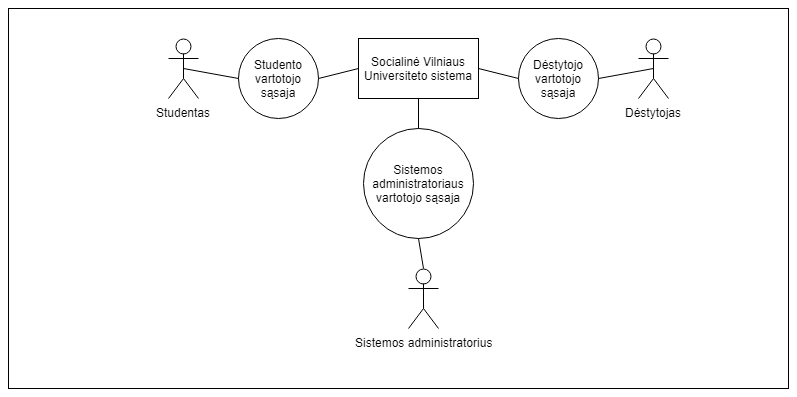
\includegraphics[width=\linewidth]{img/0lygmuo.png}
	\caption{Komponentų diagramos nulinis lygmuo}
	\label{fig:0lygmuo}
\end{figure}

Komponentų diagramos nuliniame lygmenyje (19 pav.) vaizduojamas bendras komponentų vaizdas. Pagrindinis ir vienintelis šio lygio komponentas yra "Socialinė Vilniaus Universiteto sistema". Šis komponentas sąveikauja su keliomis vartotojo sąsajomis. Studento ir dėstytojo grafinė vartotojo sąsaja įgalina šiuos vartotojus naudotis sistema.

\subsection{Komponentų diagramos pirmasis lygmuo}

\begin{figure}[H]
	\centering
	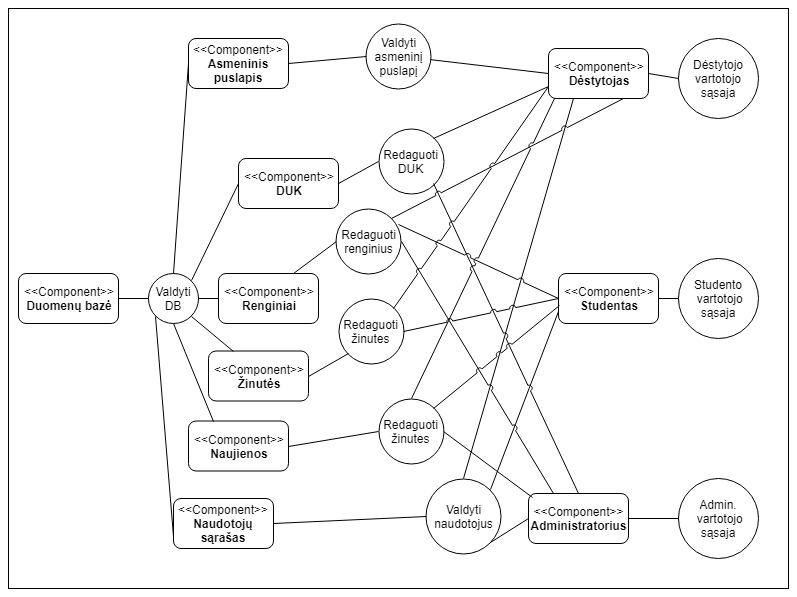
\includegraphics[width=\linewidth]{img/1lygmuo.png}
	\caption{Komponentų diagramos pirmasis lygmuo}
	\label{fig:0lygmuo}
\end{figure}

Komponentų diagramos pirmame lygmenyje komponentų diagrama yra suskaidoma. Socialinė Vilniaus universiteto sistema yra suskaidoma į šiuos komponentus: Duomenų bazė, Asmeninis puslapis, DUK, Renginiai, Žinutės, Naujienos, Naudotojų sąrašas. Šiame lygyje kiekviena vartotojo sąsaja turi už ją atsakingus komponentus. Taip pat kiekvienas komponentas turi sąsajas su kitais komponentais tam, jog galėtų vykti sąveika ir keitimasis paslaugomis. Tokiu būdu yra užtikrinama visapusiška komponentų realizacija bei tarpusavio darna.

\subsection{Komponentų diagramos antrasis lygmuo}

\begin{figure}[H]
	\centering
	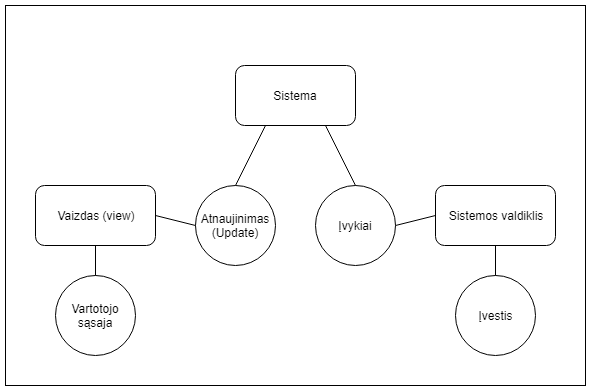
\includegraphics[width=\linewidth]{img/2lygmuo.png}
	\caption{Komponentų diagramos antrasis lygmuo}
	\label{fig:0lygmuo}
\end{figure}

Antrame lygmenyje dekomponavimui buvo pasitelktas MVC dizaino šablonas. Šis modelis buvo pasirinktas dėl jo paprastumo, universalumo ir populiarumo.
MVC šabloną sudaro trys pagrindiniai komponentai: Model, View ir Controller. Model (šiuo atveju, mūsų Sistema) – pagrindinis šablono komponentas, jis atsakingas už visos sistemos elgesį probleminėje situacijoje, nepriklausomai nuo vartotojo sąsajos, taip pat jis atsakingas už duomenis, logiką ir taisykles. Vaizdas (view) – komponentas, kuris
yra atsakingas už informacijos atvaizdavimą, jos atnaujinimą. Valdiklis – komponentas,
kuris rūpinasi duomenų įvestimi ir įvesties apdorojimu.

\newpage
\section{FIZINIS PJŪVIS}
Fizinis pjūvis sudarytas iš dislokavimo diagramų. Šiose diagramose vaizduojamas programos komponentų išdėstymas tinkle bei komunikacijos protokolai tarp jų. 
\subsection{Dislokavimo diagrama nr.1 (komponentų ir artefaktų ryšių diagrama)}
\begin{figure}[H]
	\centering
	\includegraphics[width=\linewidth]{img/compArtifacts.png}
	\caption{Komponentų ir artefaktų ryšių diagrama}
	\label{fig:compOne}
\end{figure}
Komponentų ir artefaktų ryšių diagramoje (\ref{fig:compOne}pav.) vaizduojamas artefaktas JobSys- tem.dll, kuris įgyvendina šiuos programos komponentus: Autentifikacija, Studentas, Dėstytojas, Naujienų sąrašas, Renginių sąrašas, Žinutės, Asmeninis puslapis.
\subsection{Dislokavimo diagrama nr.2 (mazgų ir artefaktų ryšių diagrama)}
\begin{figure}[H]
	\centering
	\includegraphics[width=\linewidth]{img/knotArt.png}
	\caption{Mazgų ir artefaktų ryšių diagrama}
	\label{fig:compTwo}
\end{figure}
Mazgų ir artefaktų diagramoje (\ref{fig:compTwo}pav.) parodo, kad tinklalapis yra serveryje, kuris bendrauja hhtp protokolu su SQL serveriu, kuriame saugoma duomenų bazė. Naudotojai turi galimybe pasiekti sistemos teikiamas paslaugas savo pasirinkta naršykle, kuri palaiko http protokolą.
\subsection{Dislokavimo diagrama nr.3 (mazgų ir artefaktų egzempliorių diagrama)}
\begin{figure}[H]
	\centering
	\includegraphics[width=\linewidth]{img/knotArtTwo.png}
	\caption{Mazgų ir artefaktų egzempliorių diagrama}
	\label{fig:compThree}
\end{figure}
\ref{fig:compThree}pav. vaizduojamas įrenginių (mazgų) išsidėstymas tinkle. Serveris turi tiesioginį ryšį su duomenų baze, o naudotojai gali prisijungti prie serverio. Tačiau nadotojai negali tiesiogiai pasiekti duomenų bazės ir joje saugomų duomenų.
\newpage
\section{PROCESO PJŪVIS}
Procesų pjūvis sudarytas iš sekų ir veiklos diagramų. Diagramose parodoma, kokie procesai
vyksta sistemoje bei išreiškiama komunikacija tarp jų.
\subsection{Proceso sekų diagramos}
Procesų sekų diagramose, atsispindi procesai, kurie yra vykdomi sistemoje. Iš proceso
sekų diagramos galima matyti, kokie komponentai dalyvauja vykdyme, kaip procesas vykdomas.
\subsubsection{Proceso „Prisijungimas” sekų diagrama}
\begin{figure}[H]
	\centering
	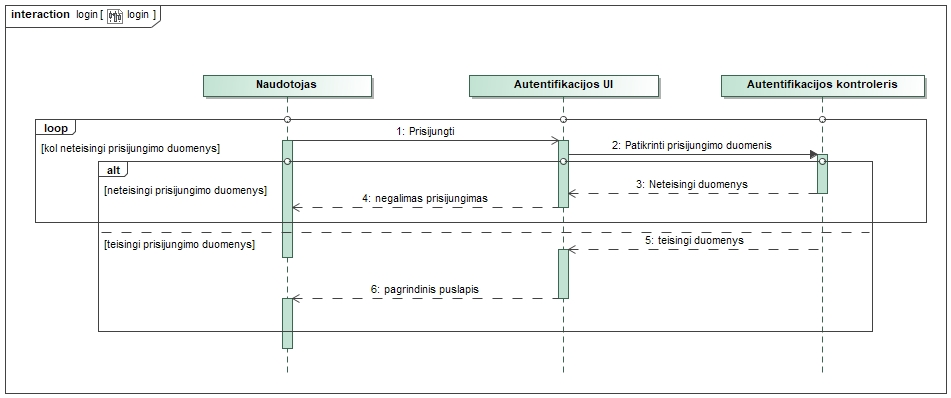
\includegraphics[width=\linewidth]{img/login.jpg}
	\caption{Proceso „Prisijungimas” sekų diagrama}
	\label{fig:login}
\end{figure}
Pagal \ref{fig:login} pav. diagramą matoma, kad procesas prasideda naudotojo paspaudimu ant nuorodos įgalinančios prisijungimą. Autentifikacijos
UI gautus duomenis siunčia patikrinimui į autentifikacijos kontrolerį. Iš kontrolerio
gaunamas atsakymas, ar duomenys teisingi ar ne. Jei duomenys klaidingi, naudotojui išmetamas pranešimas,
jog prisijungti negalima ir jis vėl gali kartoti prisijungimo procesą. Jei duomenys teisingi,
naudotojas yra nukreipiamas į pagrindinį puslapį.
\subsubsection{Proceso „Konspekto įkėlimas” sekų diagrama}
\begin{figure}[H]
	\centering
	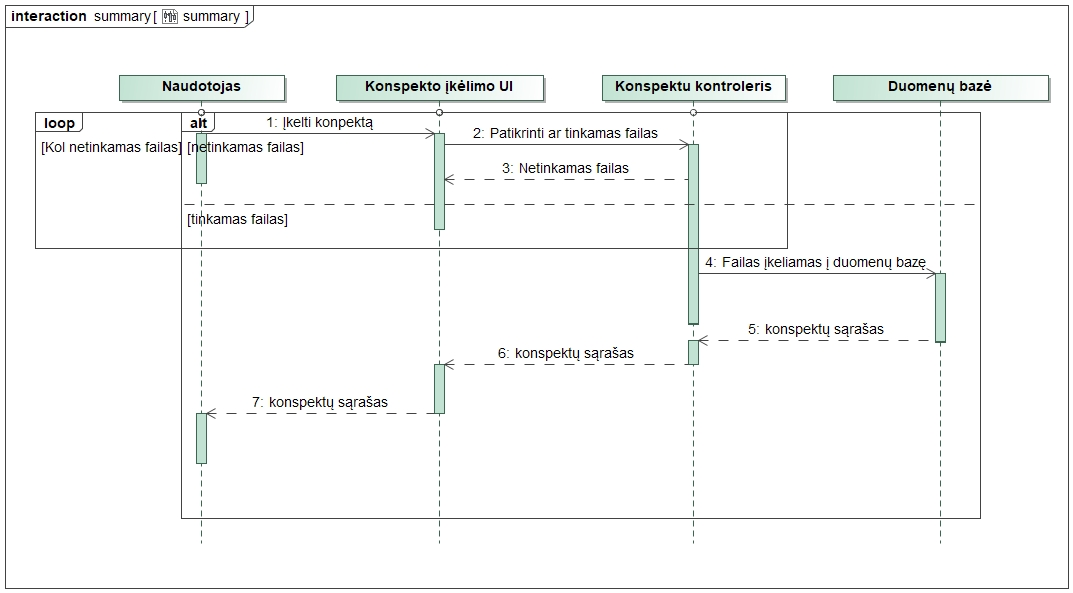
\includegraphics[width=\linewidth]{img/summary.jpg}
	\caption{Proceso „Konspekto įkėlimas” sekų diagrama}
	\label{fig:summary}
\end{figure}
Pagal \ref{fig:summary} pav. diagramą matoma, kad procesas prasideda naudotojo paspaudimu ant nuorodos įgalinančios konspekto įkėlimą. Konpekto įkėlimo UI gautus duomenis siunčia patikrinimui į konspektų kontrolerį. Iš kontrolerio
gaunamas atsakymas, ar failas tinkamas ar ne. Jei failas netinkamas, naudotojui išmetamas pranešimas,
jog failas netinkamas ir jis vėl gali kartoti konspekto įkėlimo procesą. Jei failas tinkamas, jis yra įkeliamas į duomenų bazę, o
naudotojas yra nukreipiamas į konspektų puslapį.
\subsection{Veiklos diagramos}
Veiklos diagramos padeda suprasti dinaminį sistemos
veikimą, parodo, kokie veiksmai atliekami vykdant konkrečią veiklą, galimus vykdymo atvejus.
\subsubsection{Žinutės išsiuntimo veiklos diagrama}
\begin{figure}[H]
	\centering
	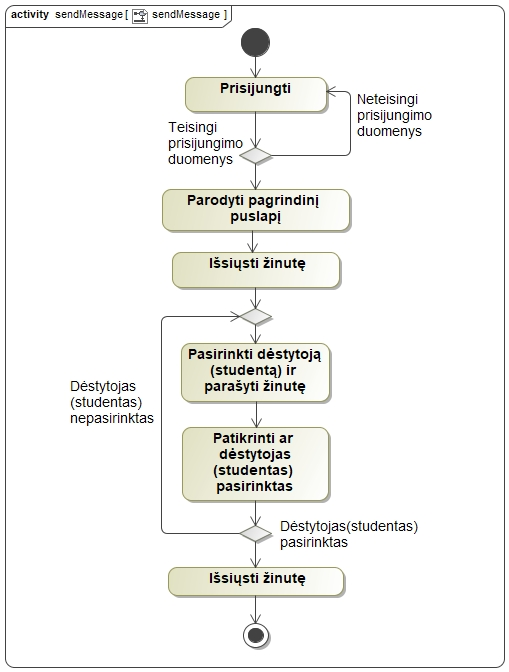
\includegraphics[scale=0.65]{img/sendMessage.jpg}
	\caption{Žinutės išsiuntimo veiklos diagrama}
	\label{fig:sendMessage}
\end{figure}
\ref{fig:sendMessage} pav. diagramoje matomas, žinutės išsiuntimo dėstytojui procesas. Procesas prasideda naudotojo
nuorodos paspaudimu, kreipiančios į žinutės išsiuntimo formą. Naudotojas pateikia parašo žinutę bei pasirenka dėstytoją, tuomet duomenys siunčiami patikrinimui. Jei dėstytojas nebuvo pasirinktas, naudotojas nukreipiamas
atgal į žinutės siuntimo formą. Jei duomenys atitinka visus reikalavimus, tada žinutė išsiunčiama.
\subsubsection{Naujienos paskelbimo veiklos diagrama}
\begin{figure}[H]
	\centering
	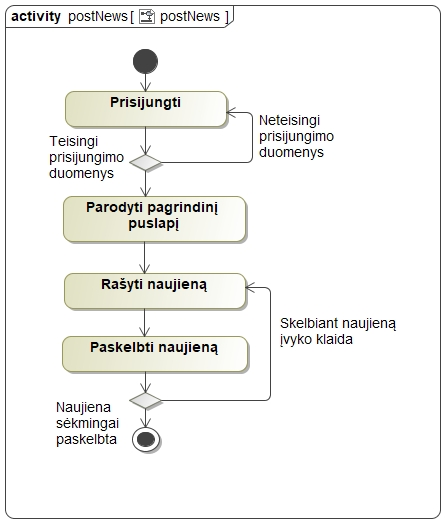
\includegraphics[scale=0.65]{img/postNews.jpg}
	\caption{Naujienos paskelbimo veiklos diagrama}
	\label{fig:postNews}
\end{figure}
\ref{fig:postNews} pav. diagramoje matomas, naujienos paskelbimo procesas. Procesas prasideda naudotojo prisijungimu. Neteisingai suvedus prisijungimo duomenis naudotojas vėl nukreipiamas į prisjungimą, kitu atveju jis nukreipiamas į pagridinį puslapį bei pasirenka naujienos paskelbimo nuorodą. Naudotojas parašo naujieną bei ją paskelbia. Jei skelbiant naujieną įvyksta klaida jis nukreipiamas į naujienos rašymo formą, kitu atveju naujiena paskelbiama.
\newpage
\sectionnonum{IŠVADOS}
Kuriamos sistemos architektūra išnagrinėta naudojant UML 4+1 požiūrių rinkinį. Iš loginio, užduočių, kūrimo, fizinio bei procesų pjūvių matome sistemos funkcionalumą, užduotis, kurias gali
įgyvendinti naudotojas, sąsajas tarp atskirų sistemos komponentų, sistemos įrangą bei dinaminį sistemos modelį.
\newpage
\sectionnonum{ŠALTINIAI}
\begin{enumerate}
\item dr. Vytautas Valaitis internetinis puslapis (https://klevas.mif.vu.lt/~valaitis/) 
\item doc., dr. Karolio Petrausko iternetinis puslapis (http://klevas.mif.vu.lt/~karolis/) 
\item https://www.magicdraw.com/files/manuals/MagicDraw Tutorials.pdf
\end{enumerate}
\end{document}